\chapter{拉普拉斯方程与泊松方程}
\intro{本章讨论椭圆型方程的基本理论，包括格林函数法和唯一性定理。}

\begin{mydefinition}{调和函数}
$u\in C^2(\Omega)$ 且在 $\Omega$ 内满足 $\lapl u=0$，则称 $u$ 为调和函数。
\end{mydefinition}

\section{基本定理}

\begin{theorem}[平均值定理]
$u$ 在球 $B_R(\vect{x}_0)$ 内调和，则
\[
u(\vect{x}_0)=\frac{1}{4\pi R^2}\oiint_{\partial B_R}u\,dS
\]
\end{theorem}

\begin{theorem}[极值原理]
$u$ 在有界区域 $\Omega$ 内调和且在 $\overline{\Omega}$ 上连续，则 $u$ 的最大值和最小值都在边界 $\partial\Omega$ 上达到。
\end{theorem}

\begin{figure}[htbp]
\centering
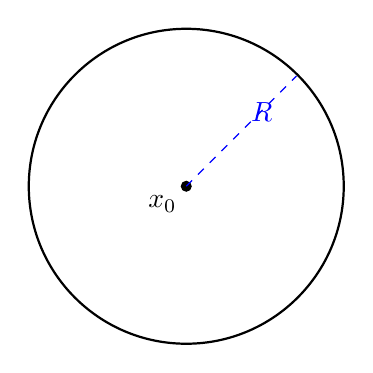
\begin{tikzpicture}
\draw[thick] (0,0) circle (2cm);
\fill (0,0) circle (2pt) node[below left]{$\vect{x}_0$};
\draw[dashed,blue] (0,0) -- (1.4,1.4) node[midway,above right]{$R$};
\end{tikzpicture}
\caption{平均值定理}
\end{figure}

\section{格林函数}

\begin{mydefinition}{格林函数}
$G(\vect{x},\vect{\xi})$ 满足：
\[
\lapl_{\vect{x}}G(\vect{x},\vect{\xi})=\delta(\vect{x}-\vect{\xi})
\]
\end{mydefinition}

\begin{theorem}[格林函数对称性]
$G(\vect{x},\vect{\xi})=G(\vect{\xi},\vect{x})$
\end{theorem}

\begin{theorem}[格林函数奇异性]
三维：$G(\vect{x},\vect{\xi})\sim\displaystyle-\frac{1}{4\pi|\vect{x}-\vect{\xi}|}$（$\vect{x}\to\vect{\xi}$）
\end{theorem}

\begin{mydefinition}{半空间格林函数（镜像法）}
上半空间 $\mathbb{R}^3_+$：
\[
G(\vect{x},\vect{\xi})=\frac{1}{4\pi}\left(\frac{1}{|\vect{x}-\vect{\xi}|}-\frac{1}{|\vect{x}-\vect{\xi}^*|}\right)
\]
其中 $\vect{\xi}^*=(\xi_1,\xi_2,-\xi_3)$。
\end{mydefinition}

\section{唯一性定理}

\begin{theorem}[Dirichlet 问题的唯一性]
$\lapl u=f$ 在 $\Omega$ 上满足相同 Dirichlet 边界条件的解唯一。
\end{theorem}

\begin{remark}
格林函数法将 PDE 求解转化为积分计算。格林函数由区域几何和边界条件类型完全决定。
\end{remark}
